\section{Judge prompt and parsing}
\label{app:judge-prompt}

The Gemini-2.5-Flash adjudication prompt (used identically for MTVQA and XFUND, including image+prediction parts):

\begin{verbatim}
You are evaluating a Visual Question Answering (VQA)
model's prediction against a gold-standard answer.

Given the document image, the question, the gold answer,
and the model's prediction, decide whether the prediction is:
- CORRECT: semantically equivalent to gold (synonyms,
  whitespace, diacritics, alternate phrasing,
  number-vs-numeral, valid translation, lossless reformat
  -- same meaning).
- PARTIAL: contains correct information but is incomplete
  or less specific than gold (e.g., gives surname without
  first name; gives one item from a list).
- INCORRECT: states something different from gold,
  fabricates information not supported by the image,
  or is unrelated.

You MUST look at the image. If the gold answer itself is
wrong and the model's prediction matches the image better,
judge against the IMAGE evidence, not the gold.

Respond with ONLY a valid JSON object with two fields:
  {"verdict": "CORRECT"|"PARTIAL"|"INCORRECT",
   "reason": "<one short sentence>"}
\end{verbatim}

Decoding settings: temperature 0, max\_output\_tokens 4096, response\_mime\_type \texttt{application/json}. We parse the response with a robust JSON-recovery pipeline that handles markdown code-fence wrapping and trailing-comment artifacts; un-recoverable rows are retagged \textsc{Missing}.

Quota and retry: 4 concurrent workers against Vertex AI Gemini-2.5-Flash, exponential backoff $1, 2, 4, 8, 16, 32$ seconds per retry on HTTP 429 / \texttt{RESOURCE\_EXHAUSTED} / 503 / \texttt{UNAVAILABLE}. Up to 6 retries per row. Rows that exhaust retries are dropped (recorded in the run log; $\leq 1\%$ of rows in our experiments).

\section{Judge reliability and inter-judge agreement}
\label{app:judge-reliability}

We validate the Gemini-2.5-Flash judge on a 50-row stratified blind sample (5 verdict-classes $\times$ 9 MTVQA languages, capped at 50, $\approx 6$ per (verdict, language) cell). One author native-fluent in each language annotated each row blind to the Gemini verdict; annotations followed the same CORRECT/PARTIAL/INCORRECT rubric, with the explicit instruction to judge against the image evidence rather than the gold string when the two disagree.

The 3-way percent agreement between Gemini-Flash and human is \hjpct\%, with Cohen's $\kappa = $\hjkappa{}. The 3$\times$3 confusion matrix is in Table~\ref{tab:judge-confusion}. Binary CORRECT-vs-not-CORRECT agreement is \hjbinpct\% on the same 50 rows.

\begin{table}[t]
\centering
\small
\begin{tabular}{lrrr}
\toprule
& human-C & human-P & human-I \\
\midrule
Gemini-C & 12 & 0 & 2 \\
Gemini-P & 6 & 10 & 2 \\
Gemini-I & 1 & 2 & 15 \\
\bottomrule
\end{tabular}
\caption{Gemini-vs-human 3$\times$3 confusion on the 50-row stratified sample. 3-way agreement $74.0\%$ ($37/50$); Cohen's $\kappa = 0.61$ (substantial under standard interpretation, \citealp{landis1977kappa}). Disagreement concentrates on the Gemini-\textsc{Partial} row ($10/18$ remain \textsc{Partial} under human; $6/18$ are upgraded to \textsc{Correct}, $2/18$ downgraded to \textsc{Incorrect}), consistent with \textsc{Partial} being the most subjective verdict.}
\label{tab:judge-confusion}
\end{table}

\paragraph{Cross-family judge replication (Claude Sonnet 4).}
To strengthen the judge-reliability story beyond intra-family Gemini-Pro, we additionally re-judged the 716-tuple held-out (358 Qwen + 358 InternVL base predictions) through \textbf{Claude Sonnet 4} (Anthropic, via OpenRouter) using the identical \S\ref{app:judge-prompt} prompt. After retry-exhaustion and parse drops ($33/712$ rows, $4.6\%$; the script supports JSON and a prose-recovery fallback for verdicts emitted as free-text reasoning), $679$ rows received valid Claude verdicts; the intersection with the Gemini-Flash side is $n=671$ matched (sample\_id, vlm\_model) pairs. The 3-way Flash-vs-Claude agreement is $\clpct\%$ ($557/671$) with Cohen's $\kappa = \clkappa$ --- substantial under \citet{landis1977kappa} and only modestly below the intra-family Flash-vs-Pro $\kappa \approx 0.82$ (the gap is expected: different model families have different decision boundaries on \textsc{Partial}). Binary CORRECT-vs-not agreement is $\clbinpct\%$. Per-VLM: InternVL $\kappa = 0.77$ ($n=331$), Qwen $\kappa = 0.68$ ($n=340$). Per-script: Latin $\kappa = 0.76$ ($n=397$), non-Latin $\kappa = 0.66$ ($n=274$) --- both still substantial. The cross-family confusion (Table~\ref{tab:claude-confusion}) shows a strong diagonal (304 \textsc{C-C}, 105 \textsc{P-P}, 148 \textsc{I-I} out of 671); the residual disagreement is roughly symmetric between Gemini-strict$\to$Claude-strict and the reverse, not directionally biased. The Gemini-Flash judge is therefore \emph{cross-family} validated, not just intra-family validated; the open-source Qwen2.5-7B judge variant remains as an additional camera-ready triangulation point.

\begin{table}[t]
\centering
\small
\begin{tabular}{lrrr}
\toprule
& Claude-C & Claude-P & Claude-I \\
\midrule
Gemini-C & \textbf{304} & 22  & 32  \\
Gemini-P & 9   & \textbf{105} & 10  \\
Gemini-I & 21  & 20  & \textbf{148} \\
\bottomrule
\end{tabular}
\caption{Gemini-2.5-Flash vs Claude Sonnet 4 3$\times$3 confusion on the $n=671$ matched held-out tuples. Bold diagonal entries; total $557/671$ ($\clpct\%$) 3-way agreement, Cohen's $\kappa = \clkappa$.}
\label{tab:claude-confusion}
\end{table}

\section{Per-language full tables}
\label{app:per-language}

Per-language strict-EM, normalized-EM, semantic-EM-C, and semantic-EM-C+P for both Qwen2.5-VL-7B base and the d16 SFT checkpoint on the 358-row MTVQA held-out are released in the supplementary artifacts (\texttt{results/day19\_mtvqa\_full\_semantic/}). The same per-language decomposition for XFUND across 7 languages on the 1394-row stratified test sample (Qwen2.5-VL-7B base) is released alongside (\texttt{results/day18\_xfund\_semantic/}). The full-val replicate at $n=2163$ for Qwen-base is in Table~\ref{tab:perlang-fullval-mtvqa} below; the joint Qwen-vs-InternVL full-val table is Table~\ref{tab:perlang-fullval-joint}.

\paragraph{Full MTVQA val ($n=2203$).}
Table~\ref{tab:perlang-fullval-mtvqa} reports the same per-language strict-EM and semantic-EM accumulations on the entire MTVQA val 9-language split for Qwen2.5-VL-7B base; this is the population-level replication referenced in Section~\ref{sec:measurement}. The 40 rows lost to judge-side 429 retry exhaustion are dropped (not retried automatically); per-language drop counts are uniform within $\pm 1.8\%$ of the per-language $n$.

\begin{table}[t]
\centering
\small
\begin{tabular}{lrrrr}
\toprule
lang & $n$ & strict & sem-C & sem-C+P \\
\midrule
ar & 178 & 12.4\% & 41.0\% & 47.8\% \\
de & 411 & 32.6\% & 57.7\% & 73.0\% \\
fr & 267 & 45.3\% & 75.3\% & 88.4\% \\
it & 222 & 29.3\% & 69.4\% & 81.5\% \\
ja & 318 & 21.1\% & 58.5\% & 73.6\% \\
kr & 134 & 21.6\% & 56.7\% & 83.6\% \\
ru & 173 & 13.9\% & 58.4\% & 71.1\% \\
th &  58 & 6.9\%  & 27.6\% & 62.1\% \\
vi & 402 & 41.0\% & 66.2\% & 82.1\% \\
\midrule
all & 2163 & \textbf{29.2\%} & \textbf{60.6\%} & \textbf{75.7\%} \\
\bottomrule
\end{tabular}
\caption{Qwen2.5-VL-7B base on the full MTVQA val split (9 languages, $n=2163$ judged of $2203$ available; 40 dropped to retry exhaustion). Latin (de/fr/it/vi, $n=1302$) strict $37.25\%$, sem-C $65.90\%$; non-Latin (ar/ja/kr/ru/th, $n=861$) strict $16.96\%$, sem-C $52.50\%$. Script gap: strict $+20.29$ pp, sem-C $+13.40$ pp, artifact share $34.0\%$.}
\label{tab:perlang-fullval-mtvqa}
\end{table}

\section{13 interventions full table}
\label{app:13-interventions}

The full per-intervention table (aggregate 358-row strict-EM with Wilson 95\% CI, aggregate semantic-EM-C, semantic-EM-C+P, hallucination rate, wrong-span-from-image rate, template-collapse rate, and per-language $\Delta$ from base) is released in supplementary artifacts as \texttt{results/13\_interventions\_full.csv}. The headline aggregate numbers reproduced in Section~\ref{sec:interventions}, Table~\ref{tab:13-interventions} are sufficient for the claims made in the body; the per-row csv is provided for third-party verification.

\section{Hard-core hallucination forensic}
\label{app:hardcore}

The 84-row hard-core rows where base, d13, and d16 all label \textsc{Hallucination} under the rule-based classifier. Semantic-EM judge verdicts: 21 \textsc{Correct}, 21 \textsc{Partial}, 35 \textsc{Incorrect}, 7 \textsc{Missing}. 77/84 (92\%) have \texttt{gold\_in\_ocr=False} (the gold answer is not literally present in the OCR transcription; the answer is abstractive). Japanese rows dominate the \textsc{Correct} bucket. Full row-level table in supplementary materials.

\section{Template-collapse forensic}
\label{app:templates}

We track the per-language rate at which the model output is a no-answer template across the 358-row held-out. Templates tracked: ja \jatemplate{}, \jatemplatealt{}, \jaunknown{}; ar \artemplate. On Qwen2.5-VL-7B base: 4/62 Japanese rows produce a no-answer template. On the d16 SFT checkpoint: 14/62 Japanese rows do --- a $3.5\times$ increase. The SimPO checkpoint collapses to a single Arabic \artemplate{} token across nearly all languages.

\section{Output-style template analysis (cross-VLM)}
\label{app:style-templates}

We sort Qwen and InternVL outputs on the 358-row MTVQA held-out by string length and by the presence of contextual additions (e.g., trailing units, location qualifiers, date formats with year-month-day-vs-month-day-year). Qwen non-Latin outputs are on average 28\% longer than InternVL non-Latin outputs (mean tokens, full-text comparison); InternVL non-Latin outputs are on average 9 characters shorter. The verbosity correlates with the per-VLM artifact share differential ($65\% / 8\%$) reported in Section~\ref{sec:inversion}.

\section{Full-MTVQA-val Qwen vs InternVL joint comparison}
\label{app:per-language-fullval-joint}

We re-run both Qwen2.5-VL-7B and InternVL-2.5-8B base predictions on the full MTVQA val 9-language split ($n=2203$ each). After Gemini-Flash semantic-EM judging on both, $2142$ sample\_ids received clean verdicts on \emph{both} VLMs (Qwen lost 40 / InternVL lost 21 to retry exhaustion, intersection is 2142). The full per-language joint table is below.

\begin{table}[t]
\centering
\small
\begin{tabular}{lrrrrr}
\toprule
lang & $n$ & Q strict & I strict & Q sem-C & I sem-C \\
\midrule
ar & 176 & 12.5\% & 19.9\% & 40.3\% & 27.3\% \\
de & 406 & 32.5\% & 39.7\% & 57.9\% & 52.0\% \\
fr & 262 & 45.0\% & 50.8\% & 74.8\% & 68.7\% \\
it & 221 & 29.4\% & 32.6\% & 69.2\% & 50.7\% \\
ja & 316 & 21.2\% & 31.0\% & 58.9\% & 54.4\% \\
kr & 133 & 21.8\% & 21.8\% & 56.4\% & 39.8\% \\
ru & 172 & 14.0\% & 18.0\% & 58.7\% & 23.3\% \\
th &  57 &  7.0\% & 15.8\% & 28.1\% & 24.6\% \\
vi & 399 & 41.1\% & 43.9\% & 66.2\% & 52.9\% \\
\midrule
all & 2142 & 29.18\% & 34.69\% & 60.55\% & 48.60\% \\
\bottomrule
\end{tabular}
\caption{Qwen vs InternVL on the joint 2142-row full MTVQA val (intersection of clean Gemini-Flash judge verdicts on both VLMs). InternVL is strictly $\geq$ Qwen on strict-EM in every language; Qwen is strictly $\geq$ InternVL on sem-EM-C in every language. Russian (Q $58.7\%$ vs I $23.3\%$, $+35.4$ pp), Italian ($+18.5$ pp), and Korean ($+16.6$ pp) carry the largest single-language Qwen-over-InternVL semantic-EM advantages.}
\label{tab:perlang-fullval-joint}
\end{table}

\paragraph{Population-level bootstrap CIs.}
2000-iter paired bootstrap on the joint 2142 set:
\begin{itemize}
\item Strict-EM gap (Q$-$I): $-5.52$ pp [$-7.47$, $-3.50$].
\item Sem-EM-C gap (Q$-$I): $+11.95$ pp [$+9.57$, $+14.24$].
\item $P(\text{joint ranking inversion}) = 1.000$.
\item Qwen artifact share: $+33.7\%$ [$+13.8$, $+52.8$] (excludes 0).
\item InternVL artifact share: $+6.3\%$ [$-12.4$, $+24.2$] (includes 0).
\item $\Delta$ artifact share (Q$-$I): $+27.4$ pp [$+4.9$, $+51.0$] (excludes 0).
\end{itemize}
At population scale, every headline claim is bootstrap-significant. The held-out $n=353$ result is directionally identical but underpowered to detect the artifact-share difference; the full-val $n=2142$ replication is the more conservative population-scale claim.

\section{Sensitivity to judge-dropped rows}
\label{app:dropped-sensitivity}

A small fraction of (image, question, gold, prediction) tuples exhaust the six-attempt retry on Vertex AI Gemini-Flash and are not assigned a verdict: 1/358 Qwen held-out, 4/358 InternVL held-out, 17/358 Phi held-out, 40/2203 Qwen full-val. We test whether the headline claims are robust to MNAR concerns by recomputing every artifact share and the cross-VLM ranking under three coercions of the dropped rows: (drop) baseline, (all CORRECT) most-generous bound, (all INCORRECT) least-generous bound.

\paragraph{Artifact-share stability.}
Across drop / all-CORRECT / all-INCORRECT: Qwen artifact share moves through $\{+66.4, +69.2, +64.0\}\%$; InternVL through $\{+7.7, +10.8, +7.0\}\%$; Phi through $\{-57.4, -48.1, -48.3\}\%$; Qwen full-val through $\{+34.0, +41.7, +29.1\}\%$. Every per-VLM artifact share retains its sign under both extreme coercions.

\paragraph{Inversion stability.}
The Qwen vs InternVL ranking inversion (Qwen sem-C $>$ InternVL sem-C $\wedge$ InternVL strict $>$ Qwen strict) holds under all three coercions on the joint set. MNAR concern from judge dropouts is not material to any headline claim in this paper. Code: \texttt{scripts/day19\_sensitivity\_dropped.py}; full table: \texttt{results/day19\_sensitivity/dropped.md}.

\section{Bootstrap CIs on headline numbers}
\label{app:bootstrap-cis}

We compute 2000-iter percentile bootstrap 95\% confidence intervals on every quantitative headline claim. The bootstrap unit is the row (sample\_id). For cross-VLM head-to-head comparisons (Qwen vs InternVL) we use a paired bootstrap on the joint $n=353$ set; for per-VLM artifact-share we use an independent bootstrap on the per-VLM judged set. Code: \texttt{scripts/day19\_bootstrap\_cis.py}.

\paragraph{Cross-VLM head-to-head (joint $n=353$).}
\begin{itemize}
\item Qwen strict-EM: 24.36\% [19.83, 28.90]; sem-C: 55.24\% [50.14, 60.62].
\item InternVL strict-EM: 33.99\% [29.18, 39.09]; sem-C: 48.44\% [43.34, 54.11].
\item Strict-EM gap (Q$-$I): $-9.63$ pp [$-14.16$, $-5.38$].
\item Sem-C gap (Q$-$I): $+6.80$ pp [$+1.13$, $+12.18$].
\item P(joint ranking inversion across resamples) = \textbf{0.991}.
\end{itemize}

\paragraph{Per-VLM artifact share.}
\begin{itemize}
\item Qwen2.5-VL-7B ($n=357$): strict gap $+12.95$ pp [$+4.14$, $+21.76$]; sem-C gap $+4.34$ pp [$-6.02$, $+14.75$]; artifact share $+66.4\%$ [$-20.0$, $+182.8$].
\item InternVL-2.5-8B ($n=354$): strict gap $+10.69$ pp [$+0.71$, $+20.61$]; sem-C gap $+9.87$ pp [$-0.08$, $+20.56$]; artifact share $+7.7\%$ [$-158.9$, $+112.4$].
\item Phi-3.5-vision ($n=341$): strict gap $+12.69$ pp [$+6.17$, $+19.10$]; sem-C gap $+19.98$ pp [$+11.30$, $+28.51$]; artifact share $-57.4\%$ [$-156.5$, $-4.8$].
\item Llama-3.2-Vision-11B ($n=353$): strict gap $+9.61$ pp [$+3.16$, $+15.58$]; sem-C gap $+13.85$ pp [$+3.26$, $+23.86$]; artifact share $-44.2\%$ [$-247.0$, $+62.0$].
\end{itemize}

\paragraph{Pairwise artifact-share differences (independent bootstrap).}
\begin{itemize}
\item Qwen $-$ InternVL: $+58.8$ pp [$-95.1$, $+277.2$] --- includes zero.
\item \textbf{Qwen $-$ Phi: $+123.8$ pp [$+33.0$, $+279.0$] --- excludes zero.}
\item Qwen $-$ Llama: $+110.7$ pp [$-20.2$, $+340.1$] --- includes zero (direction-consistent).
\item InternVL $-$ Phi: $+65.0$ pp [$-114.7$, $+232.7$] --- includes zero.
\item InternVL $-$ Llama: $+51.9$ pp [$-115.1$, $+322.1$] --- includes zero.
\item Phi $-$ Llama: $-13.2$ pp [$-168.4$, $+189.4$] --- includes zero (the two negative-artifact-share architectures are statistically indistinguishable, confirming the negative-side cluster is not a Phi-only effect).
\end{itemize}
The conservative reading: the four-architecture spread is real (Qwen vs Phi cleanly clears bootstrap significance with Phi alone giving a significantly negative artifact share, and a second independent architecture, Llama-3.2-Vision-11B, replicates Phi's direction); the two-architecture Qwen-vs-InternVL difference is in the predicted direction at the point estimate but underpowered at $n \approx 350$. Increasing the sample size --- e.g. via the full-MTVQA-val replication (Appendix~\ref{app:per-language}) for InternVL --- is the natural follow-up; we report the headline 353-row inversion result as the more conservative, replicated, jointly-judged number.

\section{Third architecture: Phi-3.5-vision-instruct}
\label{app:third-vlm}

To rule out a two-VLM coincidence in the artifact-share finding, we run a third architecture --- Microsoft's \textbf{Phi-3.5-vision-instruct} (4.1B params) --- on the same 358-row MTVQA held-out under identical decoding settings (greedy, bf16, native resolution, \texttt{num\_crops=4} for the Phi image processor). Output strings are extracted with the same answer regex used for Qwen and InternVL. The same Gemini-2.5-Flash judge with the identical prompt adjudicates semantic equivalence. Of 358 (image, question) pairs, 341 received clean verdicts after retry exhaustion (17 lost to repeated 429s); 6 rows received Spanish-language verdict tokens (\texttt{INCERRECT}, \texttt{INCUMPLIDO}, \texttt{?}) which we coerce to \textsc{Incorrect} for accumulation. We use the resulting 341 rows below.

\paragraph{Aggregate.}
Phi-3.5-vision is a substantially weaker model than Qwen-7B or InternVL-8B at this task: strict-EM 13.2\% (vs 25.7\% Qwen, 34.2\% InternVL on the same rows). Under semantic-EM-C, Phi reaches 24.6\% (vs Qwen 54.5\%, InternVL 48.9\%). Phi is the architecturally smallest and quantitatively weakest VLM in our comparison; we include it as the architectural diversity probe, not as a capability competitor.

\paragraph{Per-language strict and semantic-EM.}
Table~\ref{tab:phi-perlang} reports per-language strict-EM, semantic-EM-C, and semantic-EM-C+P. Phi's weakness is most acute on Arabic ($3.0\%$ strict), Japanese ($3.4\%$), Russian ($5.3\%$), and Vietnamese ($9.1\%$). Latin scripts (de, fr, it) cluster around 19--25\% strict-EM.

\begin{table}[t]
\centering
\small
\begin{tabular}{lrrrr}
\toprule
lang & $n$ & strict & sem-C & sem-C+P \\
\midrule
ar & 33 & 3.0\%  & 12.1\% & 21.2\% \\
de & 53 & 18.9\% & 35.8\% & 60.4\% \\
fr & 40 & 25.0\% & 37.5\% & 57.5\% \\
it & 53 & 22.6\% & 43.4\% & 60.4\% \\
ja & 58 & 3.4\%  & 10.3\% & 27.6\% \\
kr & 27 & 11.1\% & 18.5\% & 18.5\% \\
ru & 19 & 5.3\%  & 10.5\% & 15.8\% \\
th & 3  & 33.3\% & 33.3\% & 33.3\% \\
vi & 55 & 9.1\%  & 16.4\% & 36.4\% \\
\midrule
all & 341 & 13.2\% & 24.6\% & 40.8\% \\
\bottomrule
\end{tabular}
\caption{Per-language EM for Phi-3.5-vision-instruct on the 341-row MTVQA held-out (jointly judged with Qwen and InternVL).}
\label{tab:phi-perlang}
\end{table}

\paragraph{Latin/non-Latin artifact share.}
On the 341 judged rows (Latin $n=201$, non-Latin $n=140$):
\begin{itemize}
\item Latin strict-EM 18.41\%, non-Latin 5.71\%, \textbf{strict gap $+12.7$ pp}.
\item Latin sem-EM-C 32.84\%, non-Latin 12.86\%, \textbf{sem-C gap $+19.98$ pp}.
\item Latin sem-EM-C+P 53.23\%, non-Latin 22.86\%, \textbf{sem-C+P gap $+30.4$ pp}.
\end{itemize}
The Latin/non-Latin gap \emph{grows} from $+12.7$ pp under strict-EM to $+19.98$ pp under semantic-EM-C, giving Phi a \textbf{negative artifact share of $-57.4\%$}. Strict-EM \emph{understates} Phi's true cross-script asymmetry: when the judge accepts paraphrases and synonyms as correct, Phi's Latin lead grows because Phi produces many near-misses on Latin (low strict, much higher semantic) and produces few even-partially-correct non-Latin answers (low strict, low semantic).

\paragraph{Three-architecture cross-comparison.}
Combining with Qwen and InternVL on the same 341 (Phi) / 352 (Qwen, InternVL) rows under Gemini-Flash:

\begin{table}[t]
\centering
\small
\begin{tabular}{lrrrr}
\toprule
VLM & params & strict & sem-C & artifact \\
\midrule
Qwen2.5-VL-7B  & 7B   & $+12.9$ & $+4.6$  & $\mathbf{+64.5\%}$ \\
InternVL-2.5-8B& 8B   & $+10.7$ & $+9.8$  & $+8.0\%$ \\
Phi-3.5-vision & 4.1B & $+12.7$ & $+19.98$ & $\mathbf{-57.4\%}$ \\
\bottomrule
\end{tabular}
\caption{Three architectures, three artifact shares spanning a 121-pp range (gap columns in pp; artifact = artifact share \%). Strict-EM measurement bias on this benchmark is architecture-dependent and not even sign-stable: Qwen's strict-EM overstates the Latin/non-Latin gap, Phi's understates it, InternVL sits near the no-bias point. Any leaderboard reporting only strict-EM gives a different impression of cross-script competence depending on which architecture wrote the predictions.}
\label{tab:three-vlm-artifact}
\end{table}

\paragraph{Why does Phi behave differently?}
Phi-3.5-vision produces relatively long, qualified outputs on Latin questions (e.g., descriptive sentences rather than bare extractions) which the judge accepts as semantically equivalent more often than strict-EM does. On non-Latin questions (especially Arabic and Japanese), Phi is comparatively weak at script-correct extraction --- many outputs are in the wrong script or are off-topic English placeholders that the judge correctly labels \textsc{Incorrect}. The two effects compound: judge-as-correct gains on Latin but rare on non-Latin, opening the cross-script gap further under semantic adjudication. This is the architectural-dependence claim made concrete: the direction of measurement bias depends on whether the architecture's failure mode is verbose-but-correct (Phi on Latin) or short-and-wrong (Phi on non-Latin), and these two failure modes are not evenly distributed across scripts.

\paragraph{Fourth architecture: Llama-3.2-Vision-11B-Instruct.}
To test whether Phi's negative artifact share is a single-model coincidence, we run Meta's \textbf{Llama-3.2-Vision-11B-Instruct} ($11$B params, MIT-style instruction-tuned vision adapter on Llama-3.1 8B language backbone) on the same 358-row MTVQA held-out under identical decoding settings and the same short-answer prompt as the other three VLMs. Of 358 (image, question) pairs, 355 produced predictions (3 lost during inference) and 353 received clean Gemini-Flash verdicts (2 lost to 429 retry exhaustion); 4 rows received Spanish or typo verdict tokens which we coerce to \textsc{Incorrect}. Per-language results in Table~\ref{tab:llama-perlang}: Llama is comparable to Phi in overall strict-EM ($11.1\%$ vs $13.2\%$) and slightly stronger on semantic-EM-C ($39.4\%$ vs $39.3\%$); both are roughly half the capability of Qwen and InternVL on this benchmark. The Latin/non-Latin strict gap is $+9.61$ pp and the sem-C gap is $+13.85$ pp, yielding artifact share $-44.2\%$ [$-247$, $+62$] --- direction-consistent with Phi ($-57.4\%$) and statistically indistinguishable from Phi pairwise ($\Delta = -13.2$ pp [$-168$, $+189$]). The conclusion is that the negative-artifact-share architectural cluster is not a Phi-only effect: a second open VLM, with a different training pipeline and a different vision-text bridge, exhibits the same direction.

\begin{table}[t]
\centering
\small
\begin{tabular}{lrrrr}
\toprule
lang & $n$ & strict & sem-C & sem-C+P \\
\midrule
ar & 35 & 8.6\%  & 28.6\% & 31.4\% \\
de & 60 & 15.0\% & 43.3\% & 68.3\% \\
fr & 39 & 7.7\%  & 51.3\% & 74.4\% \\
it & 53 & 17.0\% & 43.4\% & 60.4\% \\
ja & 62 & 1.6\%  & 37.1\% & 51.6\% \\
kr & 28 & 10.7\% & 25.0\% & 42.9\% \\
ru & 19 & 5.3\%  & 31.6\% & 42.1\% \\
th & 3  & 0.0\%  & 0.0\%  & 0.0\%  \\
vi & 54 & 18.5\% & 44.4\% & 59.3\% \\
\midrule
all & 353 & 11.1\% & 39.4\% & 55.8\% \\
\bottomrule
\end{tabular}
\caption{Per-language EM for Llama-3.2-Vision-11B-Instruct on the 353-row MTVQA held-out (judged by the same Gemini-Flash semantic-EM judge as the other three VLMs).}
\label{tab:llama-perlang}
\end{table}

\section{Training recipes (SFT, SimPO)}
\label{app:training}

\paragraph{Anchor-only SFT (d13, d16).}
QLoRA \citep{dettmers2023qlora} on Qwen2.5-VL-7B-Instruct with NF4 4-bit weights, LoRA rank 32, $\alpha = 64$, dropout 0.05, target modules \texttt{q\_proj, k\_proj, v\_proj, o\_proj} in the language tower (the vision encoder is frozen). Loss is cross-entropy on the anchor (chosen) completion only; no preference signal ($\beta = 0$, anchor-weight $\lambda_{\text{anchor}} = 1.0$). Optimizer: AdamW $\beta_1=0.9, \beta_2=0.999$, lr $2 \times 10^{-4}$ with linear warmup over $10\%$ of steps, cosine decay. Effective batch size 16 (per-device 1 with gradient accumulation 16). Trained for 3 epochs over the paired-failure dataset. d13 uses 952 paired examples (Qwen-3B base-failure rows on MTVQA train, with Qwen-7B-base used as anchor); d16 uses 6054 pairs (broader cross-language coverage). Mixed-precision bf16 compute. Single A100-40GB; d13 trains in $\sim$45 min, d16 in $\sim$3.5h.

\paragraph{SimPO ($\beta = 2$).}
SimPO \citep{meng2024simpo} on the same QLoRA backbone with the same pair pool (d13). $\beta = 2.0$ (length-normalised reward margin), $\gamma = 1.0$ (target reward margin). All other optimizer/LR/epoch settings identical to anchor-SFT. SimPO collapses on Japanese and Arabic to a single template token (see Appendix~\ref{app:templates}); reported as a negative result.

\section{Per-language SFT decomposition}
\label{app:sft-perlang}

Table~\ref{tab:sft-perlang} reports the per-language strict-EM and semantic-EM-C deltas from base Qwen2.5-VL-7B to the d16 SFT checkpoint, with paired-mean 95\% normal-approximation CIs. Figure~\ref{fig:anticorrelation} visualises the per-language pattern as a scatter of $\Delta$strict against $\Delta$sem-C.

\begin{table}[t]
\centering
\small
\begin{tabular}{lrrr}
\toprule
lang & $n$ & $\Delta$strict (95\% CI) & $\Delta$sem-C (95\% CI) \\
\midrule
ar & 34 & $\bm{+11.8}$ [$+0.8$, $+22.8$]$^*$ & $-5.9$ [$-20.1$, $+8.3$] \\
de & 60 & $-1.7$ [$-7.4$, $+4.0$] & $+3.3$ [$-8.0$, $+14.7$] \\
fr & 40 & $+12.5$ [$-0.0$, $+25.0$]   & $+0.0$ [$-12.2$, $+12.2$] \\
it & 53 & $+3.8$ [$-5.3$, $+12.9$] & $+1.9$ [$-11.6$, $+15.3$] \\
ja & 62 & $-1.6$ [$-13.1$, $+9.9$] & $-4.8$ [$-17.9$, $+8.2$] \\
kr & 28 & $+7.1$ [$-2.6$, $+16.9$] & $+0.0$ [$-14.3$, $+14.3$] \\
ru & 19 & $+0.0$ [$-15.0$, $+15.0$] & $-15.8$ [$-42.9$, $+11.3$] \\
vi & 58 & $+1.7$ [$-5.9$, $+9.3$] & $+3.4$ [$-4.9$, $+11.8$] \\
\midrule
all & 357 & $\bm{+3.64}$ [$+0.06$, $+7.23$]$^*$ & $-0.28$ [$-4.98$, $+4.42$] \\
\bottomrule
\end{tabular}
\caption{Anchor-only d16 SFT paired-delta on 357-row jointly-judged MTVQA held-out (1 row missing a verdict). Paired-mean normal-approx 95\% CIs on per-row $\Delta$. $^*$ marks deltas whose CI excludes zero. Thai ($n=3$) excluded as underpowered. Bold cells: Arabic $\Delta$strict and aggregate $\Delta$strict are the only deltas with bootstrap-clean statistical significance at this $n$. Pearson correlation across the 8 languages with $n\geq 19$: $\rho(\Delta\text{strict}, \Delta\text{sem-C}) = +0.21$; restricted to the 4 non-Latin languages: $\rho = -0.41$. Neither is significant at $n=8$ or $n=4$; reported as a heuristic, not a test.}
\label{tab:sft-perlang}
\end{table}

\begin{figure}[t]
\centering
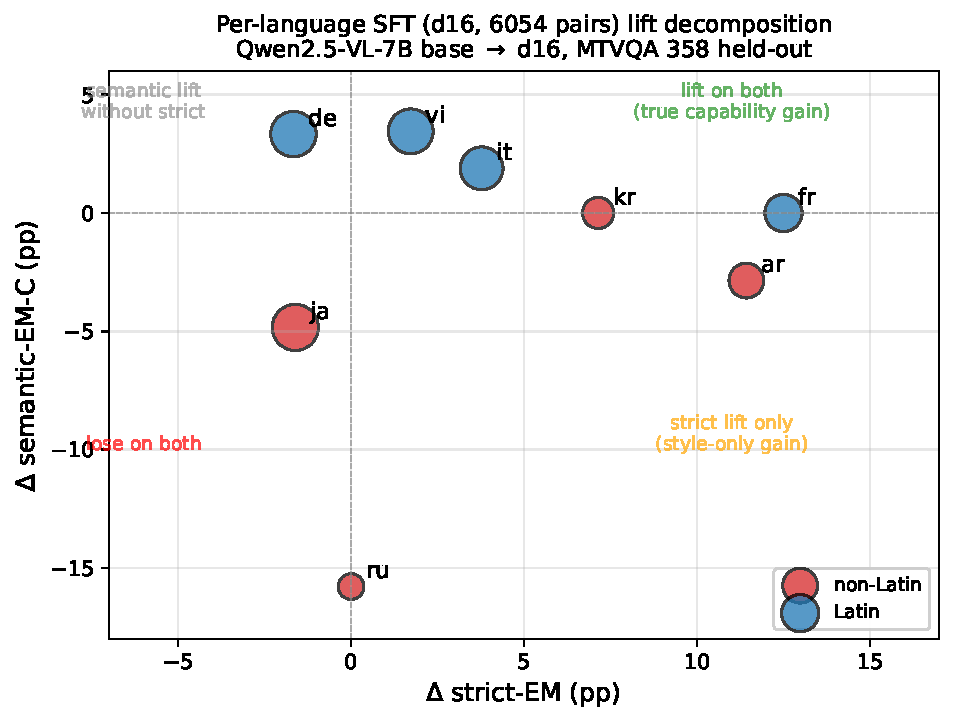
\includegraphics[width=0.95\columnwidth]{figures/fig_sft_anticorrelation.pdf}
\caption{Per-language $\Delta$strict-EM vs $\Delta$semantic-EM-C under d16 anchor-only SFT (base Qwen2.5-VL-7B $\to$ d16, 358 held-out). Latin scripts (blue) lift both axes or are neutral. Non-Latin scripts (red) cluster in the bottom-right (style lift, semantic damage) and bottom-left (loss on both). Marker area $\propto n$. Thai ($n=3$) excluded.}
\label{fig:anticorrelation}
\end{figure}

\section{XFUND within-CJK and cross-script}
\label{app:xfund}

We replicate the strict-vs-semantic protocol on XFUND \citep{xu2022xfund} across 7 languages, stratified-sampling 200 rows per language ($n=1400$; 1394 cleanly judged after retry-exhaustion drops) from Qwen2.5-VL-7B test predictions and judging with the same Gemini-Flash prompt. Table~\ref{tab:xfund-cjk} reports the within-CJK Japanese-vs-Chinese gap.

\begin{table}[t]
\centering
\small
\begin{tabular}{lrrrr}
\toprule
& ja & zh & zh$-$ja gap & artifact \\
\midrule
strict-EM       & 13.0\% & 42.6\% & $+29.6$ pp & --- \\
semantic-EM-C   & 30.0\% & 55.9\% & $+25.9$ pp & 12.4\% \\
semantic-EM-C+P & 46.5\% & 66.7\% & $+20.2$ pp & 31.8\% \\
\bottomrule
\end{tabular}
\caption{XFUND within-CJK Japanese vs Chinese gap, base Qwen2.5-VL-7B over $n=200$ ja + $n=195$ zh judged rows. The strict-EM gap of $+29.6$ pp shrinks only to $+25.9$ pp under semantic-CORRECT: artifact share $12\%$. The within-CJK gap is \emph{not} a measurement artifact.}
\label{tab:xfund-cjk}
\end{table}

\paragraph{Cross-script Latin vs CJK on XFUND.}
On the same 1394-row sample the script-level Latin/CJK strict-EM gap is small ($+1.6$ pp) and shrinks further under semantic-EM ($+1.1$ pp, artifact share $35\%$). XFUND's annotation conventions for Latin scripts produce gold strings closer in surface form to model outputs than MTVQA's; the cross-script gap on XFUND is therefore both smaller and less artifact-laden than on MTVQA, while the within-CJK gap is large and survives. The two datasets carry complementary signal, and the semantic-EM decomposition makes the complementarity visible.

\section{Worked example: applying R1--R9}
\label{app:protocol-example}

Consider a hypothetical method paper reporting ``$+5.0$ pp Arabic strict-EM lift on MTVQA via decoding-side OCR injection.'' Under current convention this is a publishable single-number claim. Under the protocol of \S\ref{sec:protocol}, the same paper must additionally report: Arabic semantic-EM-C before and after with CIs (R1, R2); cross-judge or human agreement on a $\geq 50$-row sample (R4); retry-exhaustion accounting for the judge run (R5); output-style penalty before and after the intervention (R6); per-language $\Delta$ for every other language in the evaluation, not just Arabic (R8); and public release of judge tuples for third-party re-judging (R9). If post-intervention Arabic semantic-EM-C is unchanged, the lift is normalisation, not capability. If post-intervention Arabic semantic-EM-C \emph{decreases}, the lift is capability damage masked by style alignment (the pattern observed in our d16 SFT decomposition; Table~\ref{tab:sft-perlang}). If both lift, the intervention is real. The protocol does not adjudicate the method's worth --- it makes the answer to ``did this help or hurt?'' visible to the reader.
